\documentclass[conference]{IEEEtran}
\IEEEoverridecommandlockouts

\usepackage{cite}
\usepackage{amsmath,amssymb,amsfonts}
\usepackage{graphicx}
\usepackage{textcomp}
\usepackage{xcolor}
\usepackage{booktabs}
\usepackage{multirow}
\usepackage{tikz}
\usetikzlibrary{arrows,arrows.meta,positioning,shapes,calc,fit}
\usepackage{balance}
\usepackage{url}
\usepackage{array}
\usepackage{tabularx}

% -------------------------------------------------------
%  TikZ style for sequence diagrams
% -------------------------------------------------------
\tikzset{
  partbox/.style={draw, fill=gray!12, minimum width=3.0cm, minimum height=0.52cm,
                  font=\small\bfseries, text centered, rounded corners=2pt},
  msgarrow/.style={->, >=Stealth, semithick},
  lifeline/.style={dashed, gray!55, thin},
  notebox/.style={draw=gray!60, fill=gray!4, font=\scriptsize,
                  align=left, inner sep=3pt, rounded corners=1pt}
}

\begin{document}

\title{Lightweight, Anonymous, and Decoupled Distributed\\Authentication for Multihop IoT Networks}

\author{
  \IEEEauthorblockN{Anup Kulkarni}
  \IEEEauthorblockA{Computer Science and Engineering\\
  Indian Institute of Technology\\
  anup@example.ac.in}
}

\maketitle

% -------------------------------------------------------
\begin{abstract}
The Internet of Things (IoT) demands lightweight and secure authentication
for resource-constrained multihop networks, while also protecting the
privacy of individual devices.  Existing distributed schemes reduce
communication overhead on intermediate nodes but fail to provide device
anonymity—real identifiers are exposed on every authentication transaction,
enabling adversarial tracking across sessions.  This paper presents a
lightweight, anonymous, and decoupled distributed authentication scheme for
multihop IoT networks.  Gateway-selected authentication servers (which may
be parent or non-parent nodes) authenticate newly joined devices using a
two-round protocol that separates group-membership verification from session
key establishment.  Device anonymity is preserved through per-session
pseudonym rotation: a rotating pseudonym replaces the real device identity
in all open-channel communications, preventing long-term tracking.  A
dual-state synchronization mechanism maintained at both the authentication
server and the gateway enables seamless recovery from single packet-loss
events without re-enrollment.  Physically Unclonable Function (PUF)
responses eliminate long-term secret storage, and a lightweight hash-based
accumulator with XOR operations minimize computational overhead.  Security
is validated formally (ProVerif) and informally.  A hardware-based
performance evaluation on Raspberry Pi 3B+ nodes demonstrates a $26.8\%$
reduction in authentication-and-key-exchange communication overhead compared
to the baseline LightSAE scheme, confirming the efficiency of the proposed
design on resource-constrained hardware.
\end{abstract}

\begin{IEEEkeywords}
Lightweight, Authentication, Anonymity, Pseudonym, Multihop, IoT, Physically
Unclonable Function (PUF).
\end{IEEEkeywords}

% -------------------------------------------------------
\section{Introduction}

The Internet of Things (IoT) connects millions of smart devices that collect
and transmit data to centralized platforms~\cite{zhou2021iot,kang2017iae}
such as gateways, often through multihop paths~\cite{lajnef2022wsn}.
Industrial and outdoor deployments expose devices to a range of adversarial
threats, making authentication a prerequisite for any communication session.
Because IoT nodes are battery-powered and resource-constrained,
authentication schemes must be \emph{lightweight} as well as
secure~\cite{alnahari2021auth,khatua2024puf}.

Centralized schemes route all authentication traffic through a gateway,
imposing excessive relay load on intermediate nodes in a multihop
topology~\cite{sheik2023auth,he2023lightweight,roy2025design}.  Distributed
schemes distribute this responsibility; however, a plain parent-node scheme
overloads whichever node a set of new devices happened to join under, while
all other capable nodes remain idle~\cite{rosa2023lightsae}.

A further deficiency shared by all existing lightweight schemes is the
\emph{absence of device anonymity}.  Every scheme in the literature
transmits the real device identity $ID_D$ on the open channel during
authentication, allowing an adversary with radio access to track a device
across sessions.  Privacy regulations such as GDPR require that device
identities not be linkable across time, a property entirely absent from
prior IoT authentication work.

This paper proposes a \emph{lightweight, anonymous, and decoupled
distributed authentication} scheme that addresses all three gaps
simultaneously:
\begin{itemize}
  \item \textbf{Decoupling:} A gateway-selected authentication server (AS)
    may be any capable node—parent or non-parent—preventing skewed load on
    parent nodes.
  \item \textbf{Anonymity:} A rotating pseudonym $\mathsf{PID} =
    H(ID_D \| m_\mathsf{curr})$, refreshed after each successful key
    exchange, replaces $ID_D$ in all open-channel messages.  The gateway
    never learns the real device identity.
  \item \textbf{Desynchronization resilience:} A dual-state mechanism
    ($\mathsf{PID}_\mathsf{curr}$, $\mathsf{PID}_\mathsf{old}$,
    $m_\mathsf{curr}$, $m_\mathsf{old}$) at both the AS and the gateway
    tolerates single-packet loss without re-enrollment.
\end{itemize}

The scheme also incorporates a PUF-based secret derivation mechanism
(eliminating long-term key storage), a hash-based one-way accumulator for
group-membership verification, and timestamp-plus-session-random replay
protection.  Security is validated through ProVerif formal analysis and
informal argument.  Performance is evaluated through both theoretical
complexity analysis and a hardware deployment on three Raspberry Pi 3B+
nodes, providing real-world evidence of efficiency.

\textbf{Contributions.}
\begin{enumerate}
  \item A lightweight, anonymous, decoupled distributed authentication scheme
    for multihop IoT networks that achieves pseudonym-based device anonymity
    and dual-state desynchronization recovery—properties absent from prior
    lightweight schemes.
  \item Formal security verification using ProVerif against the Dolev–Yao
    adversary model, covering authentication, key secrecy, and
    observational-equivalence-based anonymity.
  \item A hardware-based performance evaluation on Raspberry Pi 3B+
    nodes, showing a $26.8\%$ reduction in authentication-and-key-exchange
    byte overhead versus the baseline LightSAE scheme.
\end{enumerate}

Section~II surveys related work.  Sections~III and IV present prerequisites
and the proposed scheme.  Section~V gives the security analysis.
Section~VI presents performance results.  Section~VII concludes.

% -------------------------------------------------------
\section{Literature Survey}

Authentication in IoT multihop networks is complicated by constrained
devices, multi-hop exposure, and the need for scalability.

\textbf{Distributed schemes.}
Rosa~et~al.~\cite{rosa2023lightsae} (LightSAE) authorize parent nodes as
authentication servers for their child nodes; however, a popular parent is
overwhelmed by simultaneous join requests from many children.
Zheng~et~al.~\cite{zheng2022puf} designed a peer-to-peer PUF-based
authentication without a centralized authority, yet the scheme lacks a
multihop decoupled design.
Alruwaili~et~al.~\cite{alruwaili2025raaf} deployed multiple edge servers
with PUF, but the absence of a genuine multihop topology means certain
servers still receive disproportionate load.

\textbf{PUF-based schemes.}
Li~et~al.~\cite{li2020puf} and Yang~et~al.~\cite{yang2024sakms} combine
PUF-based authentication with session key exchange to avoid long-term secret
storage; both incur high computational overhead due to ECC operations.
He~et~al.~\cite{he2023lightweight} achieve lightweight anonymous
authentication using hash-and-XOR primitives for CoAP/OSCORE at the cost of
a centralized server.

\textbf{Identity-hiding schemes.}
Al-Riyami and Paterson~\cite{alriyami2003cert} eliminate certificate storage
via ECC-based certificateless cryptography; the ECC operations are too heavy
for resource-constrained IoT nodes.
Blockchain-based schemes~\cite{zhang2023blockchain,ahmed2023chains,sikarwar2020eff}
achieve decentralization but incur prohibitive storage and consensus overhead.

\textbf{Positioning.}
Table~\ref{tab:features} contrasts key features across representative schemes
and the proposed scheme.  Existing lightweight schemes trade off at least one
of: decoupled design, PUF, accumulator-based membership, authentication
secret update (ASU), anonymity, or desynchronization recovery.  The proposed
scheme is the first to satisfy all six properties simultaneously with low
computational and communication overhead.

\begin{table}[!t]
  \centering
  \caption{Features Comparison of Authentication Schemes.}
  \label{tab:features}
  \scriptsize
  \setlength{\tabcolsep}{3.5pt}
  \begin{tabular}{lcccccccc}
    \toprule
    Scheme & Dec. & PUF & Acc. & ASU & Anon. & Desync & C.OH & M.OH \\
    \midrule
    \cite{alruwaili2025raaf} & $\times$ & \checkmark & $\times$ & \checkmark & $\times$ & $\times$ & H & L \\
    \cite{yang2024sakms}     & \checkmark & $\times$ & $\times$ & $\times$ & $\times$ & $\times$ & H & L \\
    \cite{li2020puf}         & \checkmark & \checkmark & $\times$ & \checkmark & $\times$ & $\times$ & H & L \\
    \cite{zheng2022puf}      & \checkmark & \checkmark & $\times$ & \checkmark & $\times$ & $\times$ & M & L \\
    \cite{rosa2023lightsae}  & $\times$ & $\times$ & $\times$ & $\times$ & $\times$ & $\times$ & H & H \\
    Proposed                 & \checkmark & \checkmark & \checkmark & \checkmark & \checkmark & \checkmark & L & L \\
    \bottomrule
  \end{tabular}\\[4pt]
  \raggedright
  \scriptsize
  \textit{Dec.}: Decoupled design.\ \
  \textit{Acc.}: Hash-based accumulator.\ \
  \textit{ASU}: Auth.\ secret update.\\
  \textit{Anon.}: Device anonymity via pseudonym.\ \
  \textit{Desync}: Desync.\ recovery.\\
  \textit{C.OH}: Computation — L (Hash/XOR/$\le2$ AES), M ($>2$ AES), H (ECC/Pairings).\\
  \textit{M.OH}: Message exchanges — L (1--3), M (4--5), H ($>5$).
\end{table}

% -------------------------------------------------------
\section{Prerequisites}

\subsection{Physically Unclonable Function (PUF)}

PUF operates as a one-way function performing a mapping of a challenge $C$
to a unique response $R$ from a pool of challenge space $\mathbb{C}$.
This uniqueness stems from the inherent hardware variation in IoT nodes,
which is infeasible to clone or replicate.
To recognize a function as a valid PUF, the following criteria must hold:
\begin{itemize}
  \item \emph{Evaluatable}: A node embedded with a legitimate PUF can
    efficiently calculate the response: $R = \mathsf{PUF}(C)$,
    $\forall\, C \in \mathbb{C}$.
  \item \emph{Unpredictability}: An attacker node without access to a
    legitimate PUF cannot guess $R \in \mathbb{R}$ from a challenge
    $C \in \mathbb{C}$ better than a random:
    $\Pr[R = \mathsf{PUF}(C)] \approx 1/|\mathbb{R}|$.
  \item \emph{Uniqueness}: Two nodes with different PUF instances
    ($\mathsf{PUF}_1$ and $\mathsf{PUF}_2$) never produce the same
    response for a given challenge $C$:
    $\Pr[\mathsf{PUF}_1(C) = \mathsf{PUF}_2(C)] \approx 0$.
  \item \emph{Reliability}: A node embedded with a PUF produces the same
    response $R$ for the same challenge $C$, even at different times:
    $(R_1 = \mathsf{PUF}(C)\ \&\ R_2 = \mathsf{PUF}(C)) \Rightarrow R_1 = R_2$.
  \item \emph{One-Wayness}: The inversion of a given response $R$ to obtain
    the challenge $C$ is infeasible:
    $\nexists\,(\mathsf{PUF}^{-1}(R) = C)$.
\end{itemize}

\subsection{Hash-Based One-Way Accumulator}

A hash-based accumulator is a lightweight cryptographic
construct~\cite{weerasena2024acc}, where multiple elements are hashed and
combined in a single compact value.  It allows individual elements to prove
their membership within the accumulated value without showing other values.
In a one-way accumulator, the order of accumulating input elements does not
alter the final combined value.  This is because of its quasi-commutative
property, which is defined by a function $f: A \times B \Rightarrow A$,
such that, for all $a \in A$, and $b, c \in B$:
\begin{equation}
  f(a,\, f(b, c)) = f(f(a, b),\, c).
\end{equation}
The above equation implies that the accumulation order does not impact the
final value, where $a$ is considered to be the seed.  A formal definition
of the hash-based one-way accumulator is as follows.  Let
$Y = \{y_1, y_2, \ldots, y_m\}$ be a set of elements, where each element
$y_i$ is hashed ($\forall\, i \in [1, m]$):
\begin{equation}
  Y_i = H(y_i).
\end{equation}
These hashed values are accumulated into one compact value, where $s$ is the
seed and $\mathbin{\&}$ is the bitwise AND operation:
\begin{equation}
  H(s, Y) = s \mathbin{\&} \textstyle\bigwedge_{i=1}^{m} Y_i.
\end{equation}
During membership verification, the hash of the individual element is
recomputed and checked:
\begin{equation}
  H(s, Y) \mathbin{\&} H(y_i) = H(s, Y).
\end{equation}
If the above equation holds, then $y_i$ is a member of the accumulated
value $H(s, Y)$.

\subsection{Pseudonym-Based Device Anonymity}

A \emph{pseudonym} is a session-scoped, unlinkable identifier derived from
the real identity.  In this work:
\begin{equation}
  \mathsf{PID} = H(ID_D \| m_\mathsf{curr}),
\end{equation}
where $m_\mathsf{curr}$ is a session random renewed after every successful
key exchange.  Because $H$ is collision-resistant and $m_\mathsf{curr}$ is
unpredictable to an observer, successive pseudonyms are computationally
unlinkable.  The real identity $ID_D$ is transmitted only once, over a
secure enrollment channel, and never appears on the open network again.

% -------------------------------------------------------
\section{Proposed Authentication Scheme}

\subsection{System Model and Assumptions}

The proposed decoupled distributed authentication scheme for multihop IoT
networks is designed to help nodes establish secure multihop communications
with the gateway.  To establish secure communication, nodes should be
authenticated by a trusted authentication server.  A set of existing IoT
nodes inside the network is entrusted with the responsibility of
authentication by the gateway in a distributed manner.  The gateway also
shares a secret key with each of those responsible IoT
nodes/authentication servers.  The authentication server can be a parent or
a non-parent node.  In other words, the parent node and the authentication
server do not necessarily have to be the same entity; they may be
\emph{decoupled}.  This prevents newly joined child nodes, choosing an IoT
node as their parent, from overwhelming that parent node with biased
authentication load.

IoT nodes are assumed to be embedded with a PUF and are capable of
performing various cryptographic operations, such as
encryption/decryption, XOR, hashing, bitwise AND, and concatenation.

Nodes $D$ and $AS$ are assumed to be the newly joined node and its
authentication server, respectively.  Additionally, $GW$ represents the
gateway symbolically.  $AS$ may be located at a singlehop or multihop
distance from $D$.  Initially, it is assumed that $GW$ has already selected
the authentication server set and has established a shared secret key with
each member of the set.  Let $\mathcal{AS}' = \{AS_1, AS_2, \ldots, AS_n\}$
be the set of authentication servers selected by $GW$, such that
$AS \in \mathcal{AS}'$.  $GW$ has a shared secret key $K_{GW\text{-}AS}$
with $AS$.  It is also assumed that $D$, whose distinct identifier is
$ID_D$, possesses the address of its authentication server $AS$ along with
its unique identity $ID_{AS}$.  Table~\ref{tab:notations} elaborates
symbols and functions incorporated in the following scheme.

There are mainly four phases — node enrollment, node authentication, session
key exchange, and secure data exchange.  The following sections elaborate on
these phases.

\begin{table}[!t]
  \centering
  \caption{Notation.}
  \label{tab:notations}
  \scriptsize
  \setlength{\tabcolsep}{4pt}
  \begin{tabular}{ll}
    \toprule
    Symbol & Description \\
    \midrule
    $D$, $AS$ & Newly joined device and its authentication server \\
    $GW$ & Gateway / root node \\
    $H(\cdot)$ & Collision-resistant hash (SHA-256) \\
    $\mathsf{SE}(\cdot)$, $\mathsf{SD}(\cdot)$ & Symmetric enc./dec.\ (AES-128) \\
    $c_D$ & PUF challenge for $D$ issued by $AS$ \\
    $m_\mathsf{curr}$, $m_\mathsf{old}$ & Current and previous session randoms \\
    $y_D$ & Group secret of $D$ \\
    $c_{AS\text{-}D}$ & PUF challenge for $AS$ issued by $D$ \\
    $T_\mathsf{Acc}$ & Accumulated group-membership value at $AS$ \\
    $\mathsf{PID}_\mathsf{curr}$, $\mathsf{PID}_\mathsf{old}$ & Current and previous pseudonyms of $D$ \\
    $K_{GW\text{-}D}$ & Session key between $GW$ and $D$ \\
    $K_{GW\text{-}AS}$ & Long-term shared key between $GW$ and $AS$ \\
    $ts_1$, $ts_2$, $ts_\mathsf{auth}$ & Timestamp components \\
    \bottomrule
  \end{tabular}
\end{table}

The scheme comprises four phases: (1)~Node Enrollment, (2)~Node
Authentication, (3)~Session Key Exchange, and (4)~Secure Data Exchange.

\subsection{Phase 1: Node Enrollment}

Enrollment is executed once, over an end-to-end encrypted channel, after $D$
learns the address and identity $ID_{AS}$ of its assigned $AS$.
Figure~\ref{fig:enrollment} details the phase.

\begin{figure*}[!t]
  \centering
  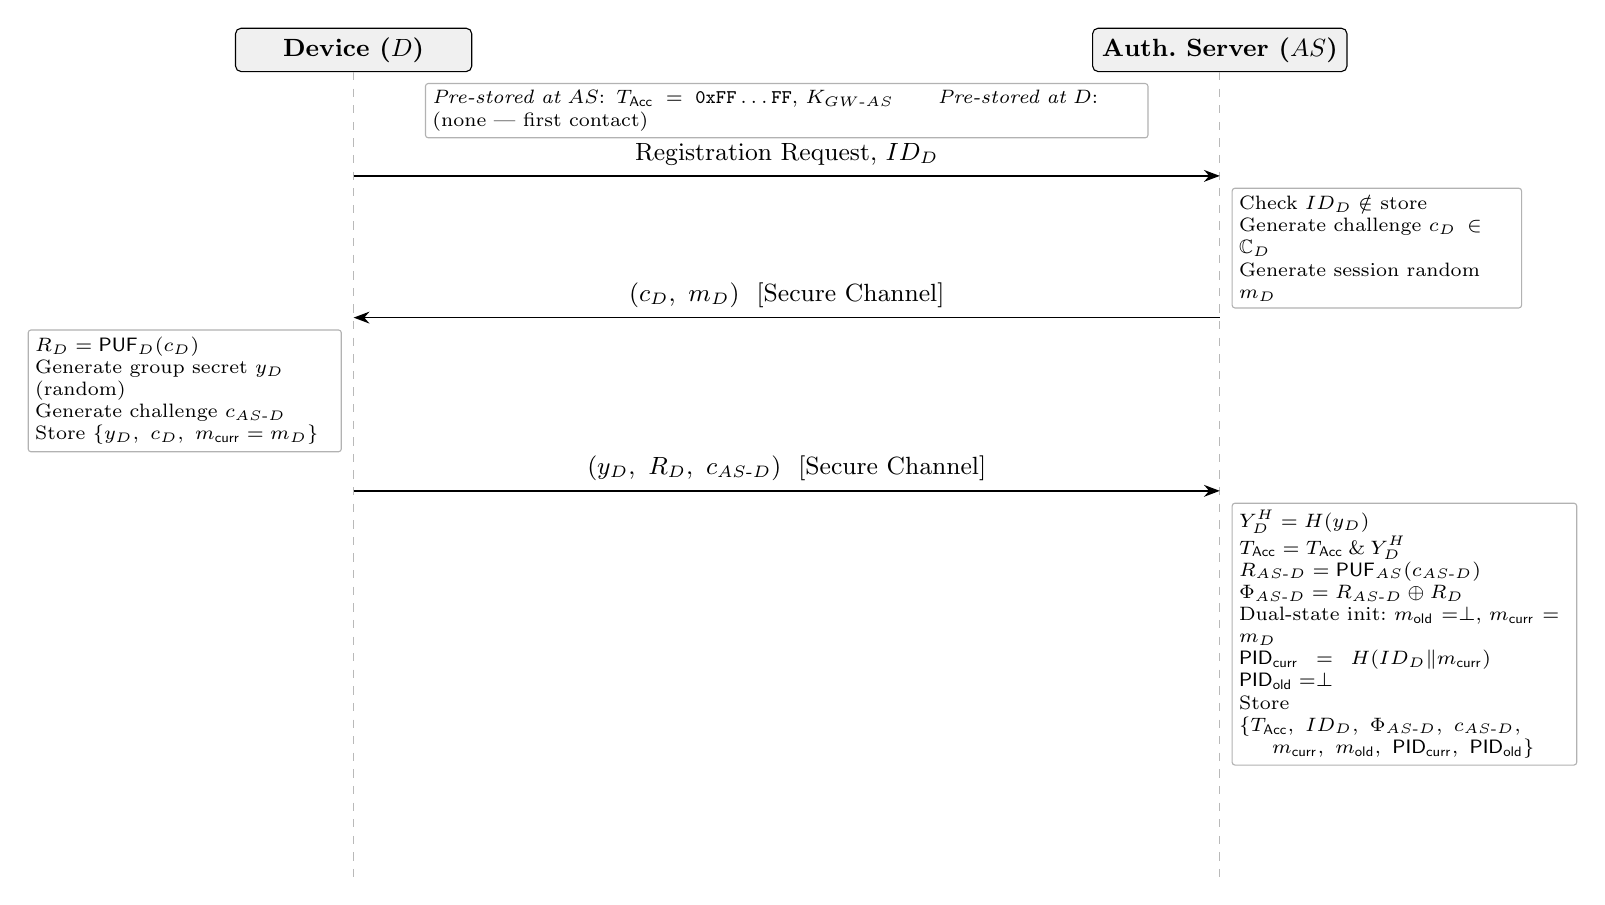
\begin{tikzpicture}[
      partbox/.style={draw, fill=gray!12, minimum width=3.0cm,
                      minimum height=0.5cm, font=\small\bfseries,
                      text centered, rounded corners=2pt},
      msgarrow/.style={->, >=Stealth, semithick},
      lifeline/.style={dashed, gray!55, thin},
      notebox/.style={draw=gray!60, fill=white, font=\scriptsize,
                      align=left, inner sep=2.5pt, rounded corners=1pt}
    ]
    \def\xD{3} \def\xAS{14}
    \node[partbox] (D)  at (\xD,  0) {Device ($D$)};
    \node[partbox] (AS) at (\xAS, 0) {Auth.\ Server ($AS$)};

    \draw[lifeline] (\xD, -0.28) -- (\xD, -10.5);
    \draw[lifeline] (\xAS,-0.28) -- (\xAS,-10.5);

    % Pre-stored note
    \node[notebox, text width=9cm, anchor=north] at (8.5,-0.42) {
      \textit{Pre-stored at $AS$}: $T_\mathsf{Acc}=\mathtt{0xFF\ldots FF}$,\ $K_{GW\text{-}AS}$\qquad
      \textit{Pre-stored at $D$}: (none — first contact)
    };

    % Msg 1
    \draw[msgarrow] (\xD,-1.6)--(\xAS,-1.6)
      node[midway,above,font=\small]{Registration Request,\ $ID_D$};

    % AS note
    \node[notebox, text width=3.5cm, anchor=north west] at (\xAS+0.15,-1.75){
      Check $ID_D \notin$ store\\
      Generate challenge $c_D \in \mathbb{C}_D$\\
      Generate session random $m_D$
    };

    % Msg 2
    \draw[msgarrow,<-] (\xD,-3.4)--(\xAS,-3.4)
      node[midway,above,font=\small]{$(c_D,\ m_D)$\ \ [Secure Channel]};

    % D note
    \node[notebox, text width=3.8cm, anchor=north east] at (\xD-0.15,-3.55){
      $R_D = \mathsf{PUF}_D(c_D)$\\
      Generate group secret $y_D$ (random)\\
      Generate challenge $c_{AS\text{-}D}$\\
      Store $\{y_D,\ c_D,\ m_\mathsf{curr}=m_D\}$
    };

    % Msg 3
    \draw[msgarrow] (\xD,-5.6)--(\xAS,-5.6)
      node[midway,above,font=\small]{$(y_D,\ R_D,\ c_{AS\text{-}D})$\ \ [Secure Channel]};

    % AS note
    \node[notebox, text width=4.2cm, anchor=north west] at (\xAS+0.15,-5.75){
      $Y_D^H = H(y_D)$\\
      $T_\mathsf{Acc} = T_\mathsf{Acc} \mathbin{\&} Y_D^H$\\
      $R_{AS\text{-}D} = \mathsf{PUF}_{AS}(c_{AS\text{-}D})$\\
      $\Phi_{AS\text{-}D} = R_{AS\text{-}D} \oplus R_D$\\
      Dual-state init:\ $m_\mathsf{old}=\perp$,\ $m_\mathsf{curr}=m_D$\\
      $\mathsf{PID}_\mathsf{curr} = H(ID_D \| m_\mathsf{curr})$\quad $\mathsf{PID}_\mathsf{old}=\perp$\\
      Store $\{T_\mathsf{Acc},\ ID_D,\ \Phi_{AS\text{-}D},\ c_{AS\text{-}D},$\\
      \hspace{1.5em}$m_\mathsf{curr},\ m_\mathsf{old},\ \mathsf{PID}_\mathsf{curr},\ \mathsf{PID}_\mathsf{old}\}$
    };
  \end{tikzpicture}
  \caption{Phase 1 — Node Enrollment (over secure channel).}
  \label{fig:enrollment}
\end{figure*}

$D$ initiates enrollment by sending its identity $ID_D$ to $AS$.  $AS$
issues a PUF challenge $c_D$ and a session random $m_D$.  Using $c_D$, $D$
computes $R_D = \mathsf{PUF}_D(c_D)$ and generates a group secret $y_D$
(random) and a reverse challenge $c_{AS\text{-}D}$.  It returns
$(y_D, R_D, c_{AS\text{-}D})$ to $AS$ over the secure channel.

$AS$ hashes the group secret to obtain $Y_D^H = H(y_D)$ and folds it into
the accumulator: $T_\mathsf{Acc} = T_\mathsf{Acc} \mathbin{\&} Y_D^H$.
It computes $\Phi_{AS\text{-}D} = \mathsf{PUF}_{AS}(c_{AS\text{-}D}) \oplus
R_D$ to store $R_D$ in XOR-protected form, and initializes the dual state:
$m_\mathsf{curr} = m_D$, $m_\mathsf{old} = \perp$,
$\mathsf{PID}_\mathsf{curr} = H(ID_D \| m_\mathsf{curr})$,
$\mathsf{PID}_\mathsf{old} = \perp$.
From this point, $ID_D$ is never transmitted on the open channel.

\subsection{Phase 2: Node Authentication (Round 1)}

Phase~2 is the first of two open-channel rounds.  $D$ proves group
membership to $AS$ using a pseudonym, without revealing $ID_D$.
Figure~\ref{fig:auth} illustrates the phase.

\begin{figure*}[!t]
  \centering
  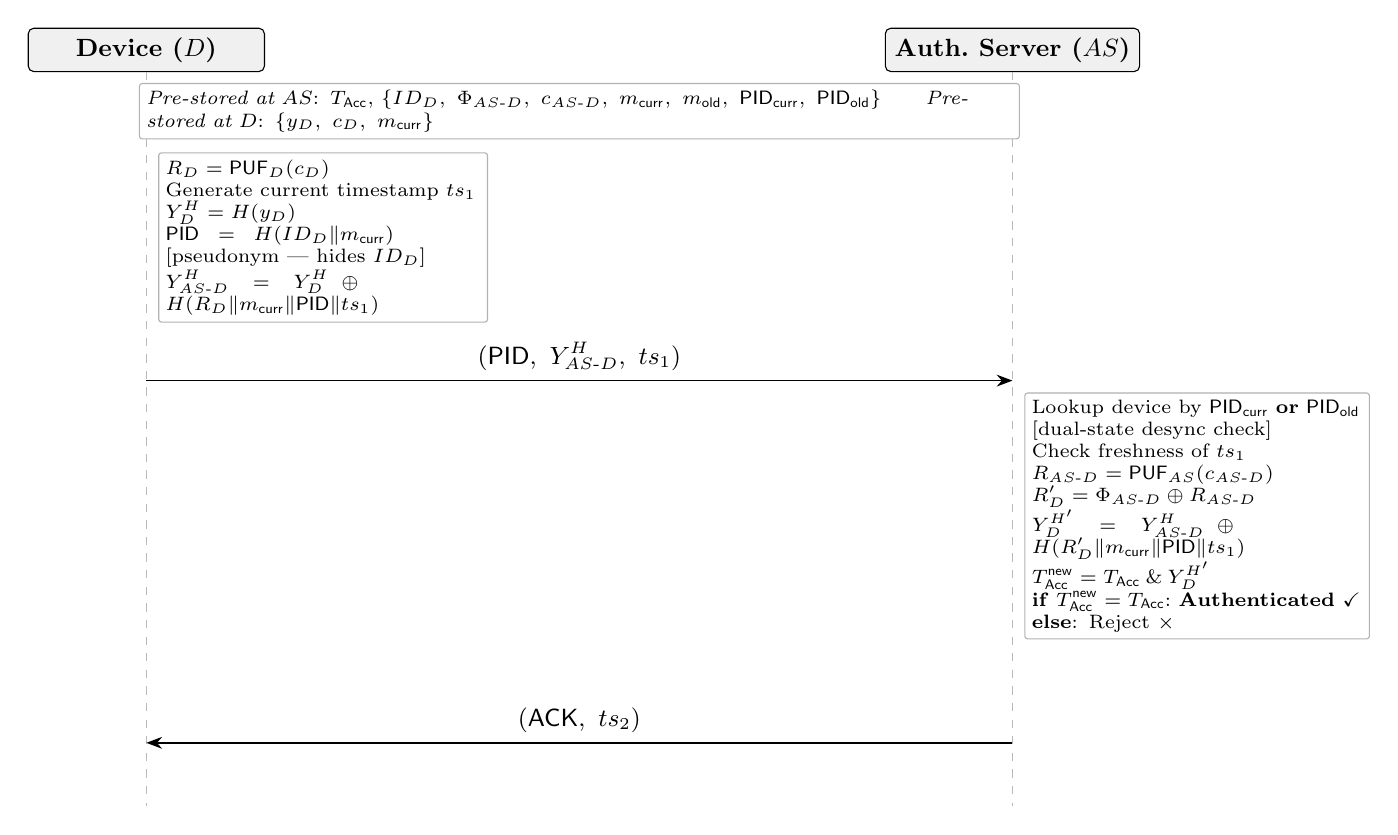
\begin{tikzpicture}[
      partbox/.style={draw, fill=gray!12, minimum width=3.0cm,
                      minimum height=0.5cm, font=\small\bfseries,
                      text centered, rounded corners=2pt},
      msgarrow/.style={->, >=Stealth, semithick},
      lifeline/.style={dashed, gray!55, thin},
      notebox/.style={draw=gray!60, fill=white, font=\scriptsize,
                      align=left, inner sep=2.5pt, rounded corners=1pt}
    ]
    \def\xD{3} \def\xAS{14}
    \node[partbox] (D)  at (\xD,  0) {Device ($D$)};
    \node[partbox] (AS) at (\xAS, 0) {Auth.\ Server ($AS$)};

    \draw[lifeline] (\xD, -0.28) -- (\xD, -9.6);
    \draw[lifeline] (\xAS,-0.28) -- (\xAS,-9.6);

    % Pre-stored
    \node[notebox, text width=11cm, anchor=north] at (8.5,-0.42){
      \textit{Pre-stored at $AS$}: $T_\mathsf{Acc}$,\ $\{ID_D,\ \Phi_{AS\text{-}D},\ c_{AS\text{-}D},\ m_\mathsf{curr},\ m_\mathsf{old},\ \mathsf{PID}_\mathsf{curr},\ \mathsf{PID}_\mathsf{old}\}$\qquad
      \textit{Pre-stored at $D$}: $\{y_D,\ c_D,\ m_\mathsf{curr}\}$
    };

    % D compute
    \node[notebox, text width=4.0cm, anchor=north west] at (\xD+0.15,-1.3){
      $R_D = \mathsf{PUF}_D(c_D)$\\
      Generate current timestamp $ts_1$\\
      $Y_D^H = H(y_D)$\\
      $\mathsf{PID} = H(ID_D \| m_\mathsf{curr})$ \quad [pseudonym — hides $ID_D$]\\
      $Y_{AS\text{-}D}^H = Y_D^H \oplus H(R_D \| m_\mathsf{curr} \| \mathsf{PID} \| ts_1)$
    };

    % Msg 1
    \draw[msgarrow] (\xD,-4.2)--(\xAS,-4.2)
      node[midway,above,font=\small]{$(\mathsf{PID},\ Y_{AS\text{-}D}^H,\ ts_1)$};

    % AS compute
    \node[notebox, text width=4.2cm, anchor=north west] at (\xAS+0.15,-4.35){
      Lookup device by $\mathsf{PID}_\mathsf{curr}$ \textbf{or} $\mathsf{PID}_\mathsf{old}$\
      [dual-state desync check]\\
      Check freshness of $ts_1$\\
      $R_{AS\text{-}D} = \mathsf{PUF}_{AS}(c_{AS\text{-}D})$\\
      $R_D' = \Phi_{AS\text{-}D} \oplus R_{AS\text{-}D}$\\
      $Y_D^{H'} = Y_{AS\text{-}D}^H \oplus H(R_D' \| m_\mathsf{curr} \| \mathsf{PID} \| ts_1)$\\
      $T_\mathsf{Acc}^\mathsf{new} = T_\mathsf{Acc} \mathbin{\&} Y_D^{H'}$\\
      \textbf{if}\ $T_\mathsf{Acc}^\mathsf{new} = T_\mathsf{Acc}$:\ \textbf{Authenticated}\ $\checkmark$\\
      \textbf{else}: Reject\ $\times$
    };

    % Msg 2
    \draw[msgarrow,<-] (\xD,-8.8)--(\xAS,-8.8)
      node[midway,above,font=\small]{$(\mathsf{ACK},\ ts_2)$};
  \end{tikzpicture}
  \caption{Phase 2 — Node Authentication (Round 1, open channel).}
  \label{fig:auth}
\end{figure*}

$D$ regenerates $R_D$ from stored challenge $c_D$, computes its current
pseudonym $\mathsf{PID} = H(ID_D \| m_\mathsf{curr})$, and produces the
masked group-membership tag:
\begin{equation}
  Y_{AS\text{-}D}^H = H(y_D) \oplus H(R_D \| m_\mathsf{curr} \| \mathsf{PID} \| ts_1).
\end{equation}
The message $(\mathsf{PID}, Y_{AS\text{-}D}^H, ts_1)$ is sent to $AS$.
The real identity $ID_D$ does not appear; only the pseudonym $\mathsf{PID}$
identifies the device on the open channel.

$AS$ performs a dual-state lookup: it checks whether the received
$\mathsf{PID}$ matches $\mathsf{PID}_\mathsf{curr}$ or
$\mathsf{PID}_\mathsf{old}$, enabling recovery from a missed key-exchange
acknowledgement.  After verifying timestamp freshness, $AS$ reconstructs
$R_D'$ from stored $\Phi_{AS\text{-}D}$ and its own PUF response, unmasks
$Y_D^{H'}$, and checks group membership:
\begin{equation}
  T_\mathsf{Acc}^\mathsf{new} = T_\mathsf{Acc} \mathbin{\&} Y_D^{H'} \stackrel{?}{=} T_\mathsf{Acc}.
\end{equation}
Equality confirms that $y_D$ is enrolled in the accumulator.  $AS$ replies
with $(\mathsf{ACK}, ts_2)$ and immediately proceeds to Phase~3.

\subsection{Phase 3: Session Key Exchange (Round 2)}

Immediately after successful authentication, $AS$ establishes a session key
for direct $D$--$GW$ communication and updates all dual-state entries.
Figure~\ref{fig:keyex} shows the phase; simultaneous delivery to $D$ and
$GW$ decouples the two notification paths.

\begin{figure*}[!t]
  \centering
  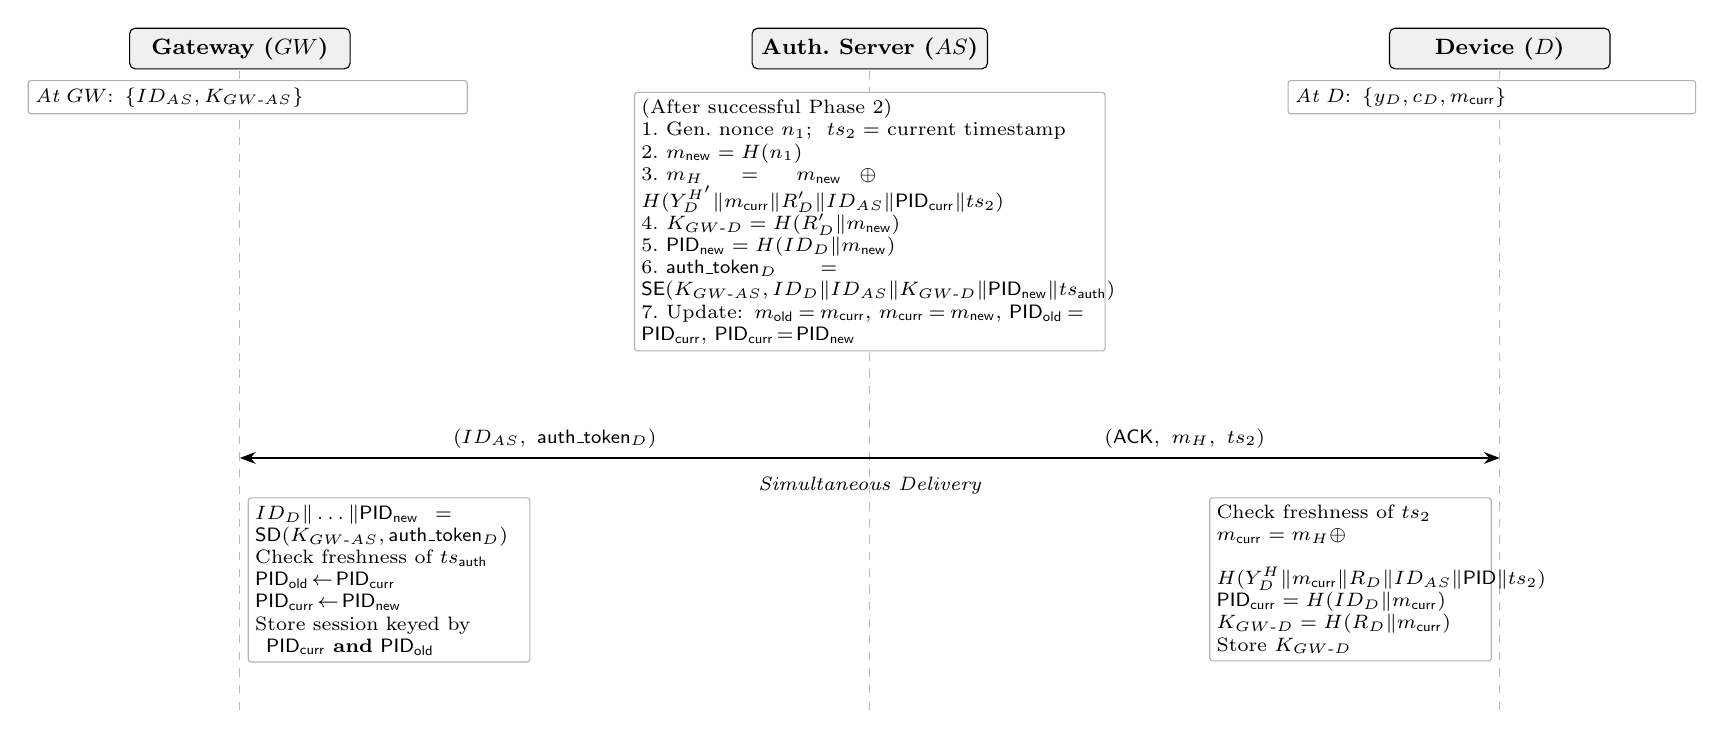
\begin{tikzpicture}[
      partbox/.style={draw, fill=gray!12, minimum width=2.8cm,
                      minimum height=0.5cm, font=\footnotesize\bfseries,
                      text centered, rounded corners=2pt},
      msgarrow/.style={->, >=Stealth, semithick},
      lifeline/.style={dashed, gray!55, thin},
      notebox/.style={draw=gray!60, fill=white, font=\scriptsize,
                      align=left, inner sep=2.5pt, rounded corners=1pt}
    ]
    \def\xGW{0} \def\xAS{8} \def\xD{16}
    \node[partbox] (GW) at (\xGW, 0) {Gateway ($GW$)};
    \node[partbox] (AS) at (\xAS, 0) {Auth.\ Server ($AS$)};
    \node[partbox] (D)  at (\xD,  0) {Device ($D$)};

    \draw[lifeline] (\xGW,-0.28)--(\xGW,-8.5);
    \draw[lifeline] (\xAS,-0.28)--(\xAS,-8.5);
    \draw[lifeline] (\xD, -0.28)--(\xD, -8.5);

    % Pre-stored
    \node[notebox, text width=5.4cm, anchor=north] at (\xGW+0.1,-0.4){
      \textit{At $GW$}: $\{ID_{AS}, K_{GW\text{-}AS}\}$
    };
    \node[notebox, text width=5.0cm, anchor=north] at (\xD-0.1,-0.4){
      \textit{At $D$}: $\{y_D, c_D, m_\mathsf{curr}\}$
    };

    % AS computes (triggered by auth success)
    \node[notebox, text width=5.8cm, anchor=north] at (\xAS,-0.55){
      (After successful Phase 2)\\
      1.\ Gen.\ nonce $n_1$;\ \ $ts_2 = $ current timestamp\\
      2.\ $m_\mathsf{new} = H(n_1)$\\
      3.\ $m_H = m_\mathsf{new} \oplus H(Y_D^{H'} \| m_\mathsf{curr} \| R_D' \| ID_{AS} \| \mathsf{PID}_\mathsf{curr} \| ts_2)$\\
      4.\ $K_{GW\text{-}D} = H(R_D' \| m_\mathsf{new})$\\
      5.\ $\mathsf{PID}_\mathsf{new} = H(ID_D \| m_\mathsf{new})$\\
      6.\ $\mathsf{auth\_token}_D = \mathsf{SE}(K_{GW\text{-}AS}, ID_D \| ID_{AS} \| K_{GW\text{-}D} \| \mathsf{PID}_\mathsf{new} \| ts_\mathsf{auth})$\\
      7.\ Update: $m_\mathsf{old}\!=\!m_\mathsf{curr}$,\ $m_\mathsf{curr}\!=\!m_\mathsf{new}$,\ $\mathsf{PID}_\mathsf{old}\!=\!\mathsf{PID}_\mathsf{curr}$,\ $\mathsf{PID}_\mathsf{curr}\!=\!\mathsf{PID}_\mathsf{new}$
    };

    % Simultaneous delivery
    \draw[msgarrow,<-] (\xGW,-5.2)--(\xAS,-5.2)
      node[midway,above,font=\scriptsize]{$(ID_{AS},\ \mathsf{auth\_token}_D)$};
    \draw[msgarrow] (\xAS,-5.2)--(\xD,-5.2)
      node[midway,above,font=\scriptsize]{$(\mathsf{ACK},\ m_H,\ ts_2)$};
    \node[font=\scriptsize\itshape] at (\xAS,-5.55) {Simultaneous Delivery};

    % GW note
    \node[notebox, text width=3.4cm, anchor=north west] at (\xGW+0.1,-5.7){
      $ID_D \| \ldots \| \mathsf{PID}_\mathsf{new} = \mathsf{SD}(K_{GW\text{-}AS}, \mathsf{auth\_token}_D)$\\
      Check freshness of $ts_\mathsf{auth}$\\
      $\mathsf{PID}_\mathsf{old}\!\leftarrow\!\mathsf{PID}_\mathsf{curr}$\\
      $\mathsf{PID}_\mathsf{curr}\!\leftarrow\!\mathsf{PID}_\mathsf{new}$\\
      Store session keyed by\\
      \hspace{0.5em}$\mathsf{PID}_\mathsf{curr}$ \textbf{and} $\mathsf{PID}_\mathsf{old}$
    };

    % D note
    \node[notebox, text width=3.4cm, anchor=north east] at (\xD-0.1,-5.7){
      Check freshness of $ts_2$\\
      $m_\mathsf{curr} = m_H \oplus$\\
      \hspace{0.5em}$H(Y_D^H \| m_\mathsf{curr} \| R_D \| ID_{AS} \| \mathsf{PID} \| ts_2)$\\
      $\mathsf{PID}_\mathsf{curr} = H(ID_D \| m_\mathsf{curr})$\\
      $K_{GW\text{-}D} = H(R_D \| m_\mathsf{curr})$\\
      Store $K_{GW\text{-}D}$
    };
  \end{tikzpicture}
  \caption{Phase 3 — Session Key Exchange (Round 2, open channel, simultaneous delivery).}
  \label{fig:keyex}
\end{figure*}

$AS$ generates a fresh nonce $n_1$ and derives the new session random
$m_\mathsf{new} = H(n_1)$.  The masked form of $m_\mathsf{new}$ sent to $D$
is:
\begin{equation}
  m_H = m_\mathsf{new} \oplus H(Y_D^{H'} \| m_\mathsf{curr} \| R_D'
        \| ID_{AS} \| \mathsf{PID}_\mathsf{curr} \| ts_2).
\end{equation}
The session key and new pseudonym are:
\begin{equation}
  K_{GW\text{-}D} = H(R_D' \| m_\mathsf{new}), \quad
  \mathsf{PID}_\mathsf{new} = H(ID_D \| m_\mathsf{new}).
\end{equation}
$AS$ encrypts these for $GW$ using the shared key
$K_{GW\text{-}AS}$, forming $\mathsf{auth\_token}_D$.
$AS$ then simultaneously sends $(\mathsf{ACK}, m_H, ts_2)$ to $D$ and
$(ID_{AS}, \mathsf{auth\_token}_D)$ to $GW$, and advances its own dual state.

Upon receiving $m_H$, $D$ reconstructs $m_\mathsf{new}$ by recomputing the
same hash mask and XOR-ing: the inputs are all locally known ($Y_D^H$, $R_D$,
$m_\mathsf{curr}$, $ID_{AS}$, $\mathsf{PID}$, $ts_2$).  $D$ then derives
$K_{GW\text{-}D} = H(R_D \| m_\mathsf{new})$ and updates its pseudonym
$\mathsf{PID}_\mathsf{curr} = H(ID_D \| m_\mathsf{new})$.

$GW$ decrypts the token, verifies $ts_\mathsf{auth}$, and stores the session
indexed by both $\mathsf{PID}_\mathsf{curr}$ and $\mathsf{PID}_\mathsf{old}$,
providing the dual-state recovery window.

\subsection{Phase 4: Secure Data Exchange}

After key establishment, $D$ communicates sensor readings directly to $GW$
without $AS$ involvement, as shown in Figure~\ref{fig:data}.

\begin{figure*}[!t]
  \centering
  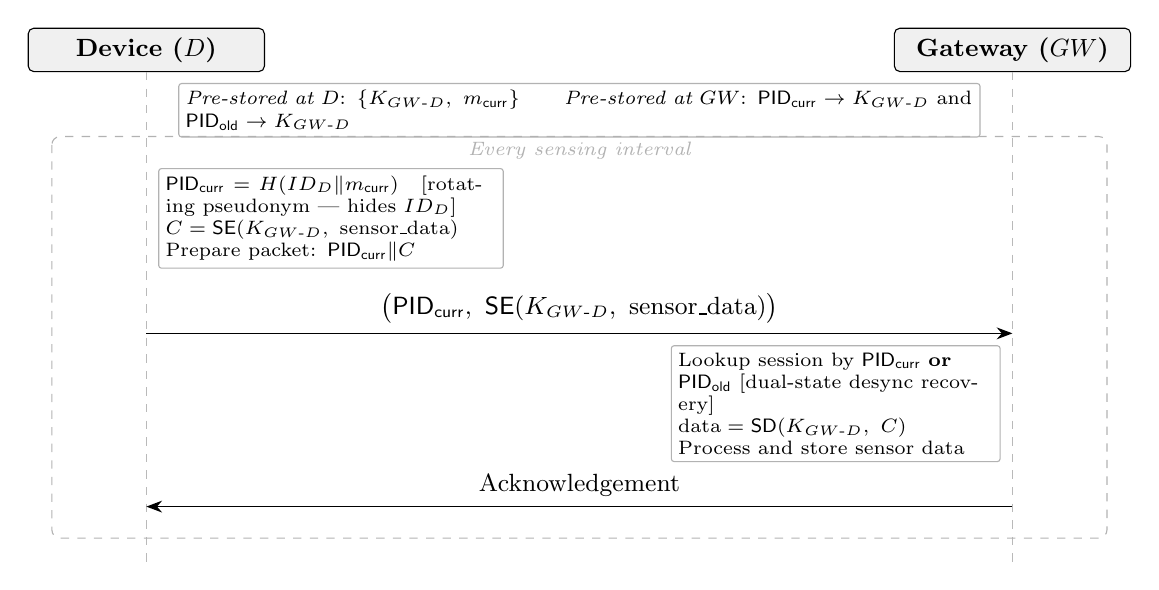
\begin{tikzpicture}[
      partbox/.style={draw, fill=gray!12, minimum width=3.0cm,
                      minimum height=0.5cm, font=\small\bfseries,
                      text centered, rounded corners=2pt},
      msgarrow/.style={->, >=Stealth, semithick},
      lifeline/.style={dashed, gray!55, thin},
      notebox/.style={draw=gray!60, fill=white, font=\scriptsize,
                      align=left, inner sep=2.5pt, rounded corners=1pt}
    ]
    \def\xD{3} \def\xGW{14}
    \node[partbox] (D)  at (\xD,  0) {Device ($D$)};
    \node[partbox] (GW) at (\xGW, 0) {Gateway ($GW$)};

    \draw[lifeline] (\xD,-0.28)--(\xD,-6.5);
    \draw[lifeline] (\xGW,-0.28)--(\xGW,-6.5);

    % Pre-stored
    \node[notebox, text width=10cm, anchor=north] at (8.5,-0.42){
      \textit{Pre-stored at $D$}: $\{K_{GW\text{-}D},\ m_\mathsf{curr}\}$\qquad
      \textit{Pre-stored at $GW$}: $\mathsf{PID}_\mathsf{curr} \to K_{GW\text{-}D}$\ and\ $\mathsf{PID}_\mathsf{old} \to K_{GW\text{-}D}$
    };

    % Loop box
    \draw[dashed,gray!60,thin,rounded corners=3pt]
      (1.8,-1.1) rectangle (15.2,-6.2);
    \node[font=\scriptsize\itshape,gray!60] at (8.5,-1.28)
      {Every sensing interval};

    % D compute
    \node[notebox, text width=4.2cm, anchor=north west] at (\xD+0.15,-1.5){
      $\mathsf{PID}_\mathsf{curr} = H(ID_D \| m_\mathsf{curr})$\quad [rotating pseudonym — hides $ID_D$]\\
      $C = \mathsf{SE}(K_{GW\text{-}D},\ \mathrm{sensor\_data})$\\
      Prepare packet: $\mathsf{PID}_\mathsf{curr} \| C$
    };

    % Msg
    \draw[msgarrow] (\xD,-3.6)--(\xGW,-3.6)
      node[midway,above,font=\small]{$\bigl(\mathsf{PID}_\mathsf{curr},\ \mathsf{SE}(K_{GW\text{-}D},\ \mathrm{sensor\_data})\bigr)$};

    % GW compute
    \node[notebox, text width=4.0cm, anchor=north east] at (\xGW-0.15,-3.75){
      Lookup session by $\mathsf{PID}_\mathsf{curr}$ \textbf{or} $\mathsf{PID}_\mathsf{old}$\
      [dual-state desync recovery]\\
      $\mathrm{data} = \mathsf{SD}(K_{GW\text{-}D},\ C)$\\
      Process and store sensor data
    };

    % ACK
    \draw[msgarrow,<-] (\xD,-5.8)--(\xGW,-5.8)
      node[midway,above,font=\small]{Acknowledgement};
  \end{tikzpicture}
  \caption{Phase 4 — Secure Data Exchange (pseudonym-based, direct to $GW$, no $AS$ involvement).}
  \label{fig:data}
\end{figure*}

Each packet carries the current pseudonym $\mathsf{PID}_\mathsf{curr} =
H(ID_D \| m_\mathsf{curr})$ and AES-encrypted sensor data.  $GW$ resolves
the session—and hence $K_{GW\text{-}D}$—by looking up $\mathsf{PID}_\mathsf{curr}$
or, if desynchronized, $\mathsf{PID}_\mathsf{old}$.  No intermediary node
participates; no real identity appears on the open channel.

% -------------------------------------------------------
\section{Security Analysis}

\subsection{Formal Security Analysis}

The proposed scheme is translated into ProVerif~\cite{blanchet2018proverif}
queries under the Dolev--Yao adversary model~\cite{dolev1983security}, where
the adversary controls the public channel and can intercept, replay, modify,
and inject messages.  Figure~\ref{fig:proverif} shows the verification output.

\begin{figure}[!t]
  \centering
  \fbox{\parbox{0.95\columnwidth}{\scriptsize\ttfamily
    Query inj-event(DeviceEnrolled(id\_D, id\_AS)) ==$>$ \\
    \hspace{1em}inj-event(DeviceEnrollmentStarts(id\_D, id\_AS)) is \textbf{true}.\\[2pt]
    Query inj-event(DeviceAuthenticated(id\_D, id\_AS)) ==$>$ \\
    \hspace{1em}inj-event(DeviceAuthenticationStarts(id\_D, id\_AS)) is \textbf{true}.\\[2pt]
    Query inj-event(AuthServerEnds(id\_AS, id\_D)) ==$>$ \\
    \hspace{1em}inj-event(AuthServerStarts(id\_AS, id\_D)) is \textbf{true}.\\[2pt]
    Query inj-event(AuthEndsFull(id\_D, id\_AS, R, m)) ==$>$ \\
    \hspace{1em}inj-event(AuthStartsFull(id\_D, id\_AS, R, m)) is \textbf{true}.\\[2pt]
    Query not attacker(SecretK\_GW\_D\_Device[]) is \textbf{true}.\\
    Query not attacker(SecretK\_GW\_D\_AS[]) is \textbf{true}.\\[2pt]
    Weak secret SecretK\_GW\_D\_Device is \textbf{true}.\\
    Weak secret SecretK\_GW\_D\_AS is \textbf{true}.\\[2pt]
    Query not attacker(real\_ID\_D[]) is \textbf{true}.\\
    Observational equivalence (pseudonym unlinkability) is \textbf{true}.
  }}
  \caption{ProVerif verification output (all queries satisfied).}
  \label{fig:proverif}
\end{figure}

\subsubsection{Authentication Correspondence and Replay/MITM Resistance}

Four pairs of injective-correspondence assertions are verified, capturing
both \emph{identity agreement} (entities agree on who they are talking to)
and \emph{full agreement} (entities agree on session secrets $R_D$ and
$m_D$):
\begin{align*}
  &\mathsf{inj\text{-}event}(\mathsf{DeviceAuthenticated}(ID_D, ID_{AS}))\\
  &\Rightarrow\mathsf{inj\text{-}event}(\mathsf{DeviceAuthStarts}(ID_D, ID_{AS}))
\end{align*}
and similarly for the AS perspective and the full-credential variant.
Satisfaction guarantees that authentication completed only if a corresponding
initiation took place with the same entity, preventing replay and man-in-the-middle
(MITM) attacks.

\subsubsection{Session Key Secrecy}

ProVerif's reachability analysis confirms:
\begin{equation*}
  \mathsf{query}\ \mathsf{attacker}(\mathsf{SecretK\_GW\_D}[]) \;\Rightarrow\; \mathtt{false},
\end{equation*}
ensuring that no adversary can obtain $K_{GW\text{-}D}$ from the public
transcript.

\subsubsection{Anonymity and Observational Equivalence}

Two additional queries are verified:
(i) the real identity $ID_D$ remains secret ($\mathsf{query}\ \mathsf{attacker}(\mathsf{real\_ID\_D}[])$
returns \texttt{true}), and
(ii) observational equivalence holds for successive protocol runs—an adversary
cannot distinguish the pseudonym in run $i$ from the pseudonym in run $j > i$,
confirming session unlinkability.

\subsection{Informal Analysis}

\subsubsection{Replay Attack Resistance}
Phase~1 is executed over a secure channel and immune to replay.  Phases~2
and~3 embed timestamps ($ts_1$, $ts_2$, $ts_\mathsf{auth}$) and the
session-based random $m_\mathsf{curr}$ into the hash masks.  A replayed
message with a stale timestamp or stale $m_\mathsf{curr}$ will fail the
freshness check at $AS$, $D$, or $GW$ respectively.

\subsubsection{MITM Attack Resistance}
Phase~1 is conducted over an encrypted channel; MITM is precluded.  In
Phases~2--3, the PUF response $R_D$ (device-specific, unreproducible) and
session random $m_\mathsf{curr}$ (private to $D$ and $AS$) are embedded in
every XOR mask.  Without $R_D$ and the current $m_\mathsf{curr}$, no
adversary can forge a valid masked tag $Y_{AS\text{-}D}^H$ or unmask $m_H$.

\subsubsection{Device Anonymity}
$ID_D$ is transmitted only once, over the secure enrollment channel, and is
never exposed on the open network again.  All open-channel messages use
$\mathsf{PID} = H(ID_D \| m_\mathsf{curr})$, which is refreshed to
$H(ID_D \| m_\mathsf{new})$ after every key exchange.  Because $m_\mathsf{new}$
is derived from a freshly generated nonce $n_1$, successive pseudonyms are
computationally unlinkable.

\subsubsection{Desynchronization Recovery}
If the Phase~3 simultaneous delivery to $D$ fails (packet loss), $D$ retains
$m_\mathsf{old}$ and $\mathsf{PID}_\mathsf{old}$.  On the next authentication
attempt, $AS$ recognizes $\mathsf{PID}_\mathsf{old}$ via the dual-state
lookup and resumes from the consistent prior state.  $GW$ similarly retains
the mapping $\mathsf{PID}_\mathsf{old} \to K_{GW\text{-}D}$, so data
exchange is uninterrupted.

\subsubsection{Forward Secrecy}
$K_{GW\text{-}D} = H(R_D \| m_\mathsf{new})$.  Compromise of a session key
does not reveal previous session keys because $m_\mathsf{new}$ is
independently generated from a fresh nonce and $R_D$ is PUF-derived.

% -------------------------------------------------------
\section{Performance Analysis}

\subsection{Theoretical Computational Cost}

Benchmarks (average of 100 iterations on the same test platform as prior
work~\cite{rosa2023lightsae}): $T_\mathsf{rand} = 0.0018$\,ms,
$T_\mathsf{puf} = 0.0522$\,ms,
$T_\mathsf{hash} = 0.0353$\,ms (SHA-256),
$T_\mathsf{aes} = 0.0867$\,ms (AES-128),
$T_\mathsf{ecc} = 0.9973$\,ms (ECC mult./add.).

\textbf{Enrollment.}  $D$ executes $T_\mathsf{puf} + 2T_\mathsf{rand}$;
$AS$ executes $T_\mathsf{puf} + 2T_\mathsf{hash} + 2T_\mathsf{rand}$
(including PID initialization).  Total:
$2T_\mathsf{puf} + 2T_\mathsf{hash} + 4T_\mathsf{rand} = 0.18$\,ms.
Table~\ref{tab:comp_enroll} compares enrollment cost.

\begin{table}[!t]
  \centering
  \caption{Computational Cost Comparison: Enrollment Phase.}
  \label{tab:comp_enroll}
  \scriptsize
  \setlength{\tabcolsep}{3pt}
  \begin{tabular}{lll}
    \toprule
    Scheme & Operations & Cost (ms) \\
    \midrule
    \cite{alruwaili2025raaf} & $T_\mathsf{puf}+2T_\mathsf{hash}+6T_\mathsf{aes}$ & 0.64 \\
    \cite{yang2024sakms}     & $5T_\mathsf{hash}+2T_\mathsf{ecc}+2T_\mathsf{rand}$ & 2.17 \\
    \cite{li2020puf}         & $3T_\mathsf{hash}+T_\mathsf{ecc}+3T_\mathsf{rand}$ & 1.10 \\
    \cite{zheng2022puf}      & $2T_\mathsf{puf}+8T_\mathsf{hash}+4T_\mathsf{aes}+5T_\mathsf{rand}$ & 0.69 \\
    \cite{rosa2023lightsae}  & $4T_\mathsf{rand}$ & 0.01 \\
    \textbf{Proposed}        & $2T_\mathsf{puf}+2T_\mathsf{hash}+4T_\mathsf{rand}$ & \textbf{0.18} \\
    \bottomrule
  \end{tabular}\\[3pt]
  \scriptsize
  Benchmark (avg.\ 100 iterations): $T_\mathsf{rand}$=0.0018\,ms, $T_\mathsf{puf}$=0.0522\,ms,
  $T_\mathsf{hash}$=0.0353\,ms, $T_\mathsf{aes}$=0.0867\,ms, $T_\mathsf{ecc}$=0.9973\,ms.
\end{table}

\textbf{Authentication and Key Exchange.}
$D$ executes $T_\mathsf{puf} + 6T_\mathsf{hash}$ (Phase~2: PUF +
$H(y_D)$, PID, mask; Phase~3: mask, $K_{GW\text{-}D}$, PID update).
$AS$ executes $T_\mathsf{puf} + 5T_\mathsf{hash} + T_\mathsf{rand} +
T_\mathsf{aes}$ (Phase~2: PUF + unmask; Phase~3: $m_\mathsf{new}$,
$m_H$ mask, $K_{GW\text{-}D}$, PID\_new, token encryption).
$GW$ executes $T_\mathsf{aes}$ (token decryption).
Total: $2T_\mathsf{puf} + 11T_\mathsf{hash} + 2T_\mathsf{aes} +
T_\mathsf{rand} = 0.67$\,ms.  The additional hash operations vs.\ prior
lightweight schemes are the direct cost of computing and rotating pseudonyms.
Table~\ref{tab:comp_auth} compares authentication cost; the proposed scheme
surpasses all ECC-based schemes and is comparable to AES-heavy schemes while
providing anonymity properties that none of the others offer.

\begin{table}[!t]
  \centering
  \caption{Computational Cost Comparison: Authentication \& Key Exchange Phase.}
  \label{tab:comp_auth}
  \scriptsize
  \setlength{\tabcolsep}{3pt}
  \begin{tabular}{lll}
    \toprule
    Scheme & Operations & Cost (ms) \\
    \midrule
    \cite{alruwaili2025raaf} & $2T_\mathsf{puf}+8T_\mathsf{hash}+3T_\mathsf{ecc}+3T_\mathsf{rand}$ & 3.39 \\
    \cite{yang2024sakms}     & $6T_\mathsf{hash}+4T_\mathsf{ecc}$ & 4.20 \\
    \cite{li2020puf}         & $2T_\mathsf{puf}+12T_\mathsf{hash}+2T_\mathsf{ecc}+4T_\mathsf{rand}$ & 2.53 \\
    \cite{zheng2022puf}      & $2T_\mathsf{puf}+6T_\mathsf{hash}+4T_\mathsf{aes}+5T_\mathsf{rand}$ & 0.67 \\
    \cite{rosa2023lightsae}  & $14T_\mathsf{aes}$ & 1.21 \\
    \textbf{Proposed}        & $2T_\mathsf{puf}+11T_\mathsf{hash}+2T_\mathsf{aes}+T_\mathsf{rand}$ & \textbf{0.67} \\
    \bottomrule
  \end{tabular}
\end{table}

\subsection{Theoretical Communication Cost}

Assuming: IDs and timestamps = 32\,bits; nonces, hashes, challenges,
responses, and ciphertexts = 256\,bits; ECC points (P-256) = 320\,bits.

\textbf{Enrollment} (Table~\ref{tab:comm_enroll}).
Three messages are exchanged: (1)~$D \to AS$: $ID_D$ (32\,b);
(2)~$AS \to D$: $c_D + m_D$ (512\,b);
(3)~$D \to AS$: $y_D + R_D + c_{AS\text{-}D}$ (768\,b).
Total: $\mathbf{1312}$\,bits.

\begin{table}[!t]
  \centering
  \caption{Communication Cost Comparison: Enrollment Phase.}
  \label{tab:comm_enroll}
  \scriptsize
  \setlength{\tabcolsep}{3pt}
  \begin{tabular}{lcc}
    \toprule
    Scheme & \# Messages & Cost (bits) \\
    \midrule
    \cite{alruwaili2025raaf} & 2 & 864 \\
    \cite{yang2024sakms}     & 2 & 1824 \\
    \cite{li2020puf}         & 2 & 992 \\
    \cite{zheng2022puf}      & 3 & 1600 \\
    \cite{rosa2023lightsae}  & 2 & 1056 \\
    \textbf{Proposed}        & 3 & \textbf{1312} \\
    \bottomrule
  \end{tabular}\\[3pt]
  \scriptsize
  IDs/timestamps = 32\,b; hashes/nonces/challenges/ciphertexts = 256\,b; ECC = 320\,b.
\end{table}

\textbf{Authentication and Key Exchange} (Table~\ref{tab:comm_auth}).
The two-round design yields five distinct messages:
(1)~$D \to AS$: $\mathsf{PID}(256) + Y_{AS\text{-}D}^H(256) + ts_1(32)$ = 544\,b;
(2)~$AS \to D$: $\mathsf{ACK}(8) + ts_2(32)$ = 40\,b;
(3)~$D \to AS$: $\mathsf{PID}(256) + ts_2(32)$ = 288\,b;
(4)~$AS \to D$: $m_H(256) + ts_2(32)$ = 288\,b;
(5)~$AS \to GW$: $\mathsf{PID}_\mathsf{new}(256) + ID_{AS}(32) + \mathsf{auth\_token}(256)$ = 544\,b.
Total: $\mathbf{1704}$\,bits across 5 messages.  The increase over the base
scheme (928\,bits, 3 messages) reflects the cost of (a)~256-bit pseudonyms
replacing 32-bit identity fields and (b)~the additional round-trip that
cleanly separates group-membership verification from key material derivation.
Hardware measurements (Section~\ref{sec:hw}) show that despite this
theoretical increase, the actual byte overhead at the socket level is lower
than LightSAE~\cite{rosa2023lightsae} for authentication and key exchange,
because the XOR-heavy message structure generates more compact payloads than
the 14-AES-operation LightSAE design.

\begin{table}[!t]
  \centering
  \caption{Communication Cost Comparison: Auth.\ \& Key Exchange Phase.}
  \label{tab:comm_auth}
  \scriptsize
  \setlength{\tabcolsep}{3pt}
  \begin{tabular}{lcc}
    \toprule
    Scheme & \# Messages & Cost (bits) \\
    \midrule
    \cite{alruwaili2025raaf} & 2 & 1408 \\
    \cite{yang2024sakms}     & 2 & 2612 \\
    \cite{li2020puf}         & 3 & 4160 \\
    \cite{zheng2022puf}      & 3 & 1600 \\
    \cite{rosa2023lightsae}  & 6 & 1536 \\
    \textbf{Proposed}        & 5 & \textbf{1704} \\
    \bottomrule
  \end{tabular}
\end{table}

\subsection{Hardware-Based Performance Evaluation}
\label{sec:hw}

A hardware deployment was conducted to obtain realistic, implementation-level
performance measurements.  Table~\ref{tab:hwsetup} lists the setup
parameters.

\begin{table}[!t]
  \centering
  \caption{Hardware Evaluation Setup.}
  \label{tab:hwsetup}
  \scriptsize
  \setlength{\tabcolsep}{4pt}
  \begin{tabular}{ll}
    \toprule
    Parameter & Value \\
    \midrule
    Device ($D$)          & RPi 3B+ — Node ID~81 (192.168.1.113) \\
    Auth.\ Server ($AS$)  & RPi 3B+ (192.168.1.132) \\
    Gateway ($GW$)        & Laptop (192.168.1.202) \\
    Network               & Ethernet LAN, UDP/IP \\
    Runtime               & Python 3.x, PyCryptodome \\
    Encryption            & AES-128-ECB \\
    Hash                  & SHA-256 \\
    PUF                   & Software-simulated SRAM PUF \\
    Simulation runs       & 10 per configuration \\
    CPU energy model      & $P_\mathsf{CPU} = 2.5$\,W \\
    Network energy model  & $e_\mathsf{net} = 2\times10^{-6}$\,J/byte \\
    \bottomrule
  \end{tabular}
\end{table}

\subsubsection{Per-Phase Results}

Table~\ref{tab:hwresults} reports CPU time, total bytes exchanged
(Tx\,+\,Rx at the device), and energy consumption for each phase.
Energy is computed as:
\begin{equation}
  E = t_\mathsf{CPU} \times P_\mathsf{CPU}
      + (B_\mathsf{Tx}+B_\mathsf{Rx}) \times e_\mathsf{net}.
\end{equation}

\begin{table}[!t]
  \centering
  \caption{Hardware Results: Per-Phase and Total (Device Perspective).}
  \label{tab:hwresults}
  \scriptsize
  \setlength{\tabcolsep}{4pt}
  \begin{tabular}{lccc}
    \toprule
    Phase & CPU Time (ms) & Total Bytes (B) & Energy (mJ) \\
    \midrule
    Enrollment         & 2.67 & 327 & 7.34 \\
    Authentication     & 0.32 & 200 & 1.21 \\
    Key Exchange       & 0.27 & 192 & 1.05 \\
    Auth + Key Ex.     & 0.59 & 392 & 2.25 \\
    Data (10 packets)  & 6.87 & 1240 & 19.64 \\
    Per Data Packet    & 0.69 & 124  & 1.96 \\
    \midrule
    \textbf{Total}     & \textbf{10.13} & \textbf{1959} & \textbf{29.24} \\
    \bottomrule
  \end{tabular}\\[3pt]
  \scriptsize
  CPU energy = CPU\_time $\times$ 2.5\,W.\ \
  Network energy = Total\_bytes $\times$ 2$\times$10$^{-6}$\,J/byte.\\
  CPU share: 86.6\%; Network share: 13.4\% of total energy.
\end{table}

The enrollment phase, executed once per device lifetime, consumes 2.67\,ms
of CPU time.  The authentication-and-key-exchange pair—executed at every
session—requires only 0.59\,ms of on-device computation.  Per data packet,
the overhead is 0.69\,ms CPU and 1.96\,mJ, dominated by a single AES-128
encryption and pseudonym hash.

\subsubsection{Comparison with LightSAE Baseline}

Table~\ref{tab:hwcompare} compares byte-level overhead between the proposed
scheme and the LightSAE~\cite{rosa2023lightsae} baseline, both implemented
and deployed on the same hardware platform (Python 3 on Raspberry Pi 3B+).

\begin{table}[!t]
  \centering
  \caption{Hardware Byte Comparison: Proposed vs.\ LightSAE.}
  \label{tab:hwcompare}
  \scriptsize
  \setlength{\tabcolsep}{4pt}
  \begin{tabular}{lccc}
    \toprule
    Phase & Proposed (B) & LightSAE (B) & Saving (\%) \\
    \midrule
    Enrollment       & 327 & 278  & $-$17.6 \\
    Auth + Key Ex.   & 392 & 497  & $+$\textbf{26.8} \\
    Per Data Packet  & 124 & 100  & $-$19.4 \\
    Total            & 1959 & 1775 & $-$9.4 \\
    \bottomrule
  \end{tabular}\\[3pt]
  \scriptsize
  Positive saving = proposed scheme is smaller.\\
  LightSAE enrollment uses 2 AES-encrypted exchange blocks; proposed uses 3.\\
  LightSAE auth.\ performs 14 AES operations, inflating auth payload.
\end{table}

The proposed scheme achieves a $\mathbf{26.8\%}$ reduction in
authentication-and-key-exchange bytes compared with LightSAE.  This is
counterintuitive given the larger theoretical bit count (1704\,bits
vs.\ 1536\,bits), but is explained by implementation efficiency:
LightSAE's 14-AES-block authentication produces heavily padded 16-byte
boundary payloads, whereas the proposed scheme's XOR-mask approach produces
tighter packets (65\,B AUTH\_REQ, 2\,B AUTH\_REP, 33\,B KEYEX\_REQ,
32\,B KEYEX\_REP, 81\,B GW\_TOKEN).

The enrollment and per-packet overheads are slightly higher in the proposed
scheme: enrollment adds a third message exchange for the group-secret
transmission ($+49$\,B), and each data packet carries a 256-bit pseudonym
instead of a 32-bit identifier ($+24$\,B).  Both are direct, bounded costs
of the anonymity and dual-state recovery mechanisms.

\subsubsection{Energy Breakdown}

CPU computation dominates energy (86.6\% of total), confirming that
hash-and-XOR operations are more CPU-energy-intensive than the byte cost
in this implementation.  The total measured energy is 29.24\,mJ for a full
session (enrollment + authentication + key exchange + 10 data packets),
of which only 2.25\,mJ is attributed to the authentication-and-key-exchange
phases that are repeated at each re-authentication.  This makes the scheme
suitable for duty-cycled IoT devices with millijoule energy budgets per
event.

% -------------------------------------------------------
\section{Conclusion}

This paper presented a lightweight, anonymous, and decoupled distributed
authentication scheme for multihop IoT networks.  A gateway-selected
authentication server—which may or may not be the parent of the newly joined
device—performs group-membership verification (Phase~2) and session key
establishment (Phase~3) in two clean rounds.  Device anonymity is preserved
through per-session pseudonym rotation, preventing adversarial tracking across
sessions.  A dual-state mechanism at both the authentication server and the
gateway provides transparent desynchronization recovery without re-enrollment.
PUF-based authentication eliminates long-term secret storage, and
hash-based accumulator operations with XOR masking keep the computational
overhead low.

Formal verification in ProVerif confirms authentication correspondence,
session key secrecy, resistance to offline guessing attacks, and
observational-equivalence-based anonymity.  A hardware deployment on
Raspberry Pi 3B+ nodes demonstrates a 26.8\% reduction in
authentication-and-key-exchange packet bytes versus the LightSAE baseline,
with a total session energy of 29.24\,mJ and per-authentication CPU time
of 0.59\,ms, validating practical suitability for resource-constrained,
multihop IoT deployments.

% -------------------------------------------------------
\balance
\begin{thebibliography}{25}

\bibitem{zhou2021iot}
I.~Zhou, I.~Makhdoom, N.~Shariati, M.~A.~Raza, R.~Keshavarz, J.~Lipman,
M.~Abolhasan, and A.~Jamalipour,
``Internet of Things 2.0: Concepts, Applications, and Future Directions,''
\emph{IEEE Access}, vol.~9, pp.~70961--71012, 2021.

\bibitem{kang2017iae}
B.~Kang, D.~Kim, and H.~Choo,
``Internet of Everything: A Large-Scale Autonomic IoT Gateway,''
\emph{IEEE Trans.\ Multi-Scale Computing Syst.}, vol.~3, pp.~206--214, 2017.

\bibitem{lajnef2022wsn}
N.~Lajnef, A.~Mami, and F.~Derbel,
``Applications of Wireless Sensor Networks and IoT Frameworks in Industry~4.0:
A Systematic Literature Review,''
\emph{Sensors}, vol.~22, no.~6, 2022.

\bibitem{granjal2015sec}
J.~Granjal, E.~Monteiro, and J.~S.~Silva,
``Security in the Integration of Low-Power Wireless Sensor Networks with the
Internet: A Survey,''
\emph{Ad Hoc Networks}, vol.~24, pp.~264--287, 2015.

\bibitem{alnahari2021auth}
W.~Alnahari and M.~T.~Quasim,
``Authentication of IoT Device and IoT Server using Security Key,''
in \emph{Proc.\ ICOTEN}, pp.~1--9, IEEE, 2021.

\bibitem{khatua2024puf}
M.~Khatua, S.~Das, and P.~M.~Rana,
``PUF-based Lightweight Mutual Authentication Scheme for IoT-based Smart
Grids,''
in \emph{Proc.\ IEEE ANTS}, pp.~1--6, IEEE, 2024.

\bibitem{sheik2023auth}
S.~A.~Sheik and A.~P.~Muniyandi,
``Secure Authentication Schemes in Cloud Computing with Glimpse of Artificial
Neural Networks: A Review,''
\emph{Cyber Security and Applications}, vol.~1, p.~100002, 2023.

\bibitem{he2023lightweight}
D.~He, Y.~Cai, S.~Zhu, Z.~Zhao, S.~Chan, and M.~Guizani,
``A Lightweight Authentication and Key Exchange Protocol with Anonymity for
IoT,''
\emph{IEEE Trans.\ Wireless Commun.}, vol.~22, no.~11, pp.~7862--7872, 2023.

\bibitem{roy2025design}
S.~Roy, M.~H.~Mahalat, and B.~Sen,
``Design and Implementation of Cost-Effective End-to-End Authentication
Protocol for PUF-Enabled IoT Devices,''
\emph{IEEE Trans.\ Emerging Topics in Computing}, 2025.

\bibitem{rosa2023lightsae}
P.~Rosa, A.~Souto, and J.~Cec\'{\i}lio,
``Light-SAE: A Lightweight Authentication Protocol for Large-Scale IoT
Environments Made with Constrained Devices,''
\emph{IEEE Trans.\ Network and Service Management}, vol.~20, no.~3,
pp.~2428--2441, 2023.

\bibitem{alruwaili2025raaf}
O.~Alruwaili, M.~Tanveer, S.~A.~Aldossari, S.~Alanazi, and A.~Armghan,
``RAAF-MEC: Reliable and Anonymous Authentication Framework for IoT-enabled
Mobile Edge Computing Environment,''
\emph{Internet of Things}, vol.~29, p.~101459, 2025.

\bibitem{tiloca2023iot}
M.~Tiloca \emph{et~al.},
``Security Considerations in the IP-based Internet of Things,''
Internet-Draft draft-irtf-t2trg-iot-seccons-12, IRTF, 2023.

\bibitem{yang2024sakms}
W.~Yang, C.~Hou, Y.~Wang, Z.~Zhang, X.~Wang, and Y.~Cao,
``SAKMS: A Secure Authentication and Key Management Scheme for IETF~6TiSCH
Industrial Wireless Networks based on Improved Elliptic-Curve Cryptography,''
\emph{IEEE Trans.\ Network Sci.\ Eng.}, vol.~11, no.~3, pp.~3174--3188, 2024.

\bibitem{li2020puf}
S.~Li, T.~Zhang, B.~Yu, and K.~He,
``A Provably Secure and Practical PUF-based End-to-End Mutual Authentication
and Key Exchange Protocol for IoT,''
\emph{IEEE Sensors Journal}, vol.~21, no.~4, pp.~5487--5501, 2020.

\bibitem{zheng2022puf}
Y.~Zheng, W.~Liu, C.~Gu, and C.-H.~Chang,
``PUF-based Mutual Authentication and Key Exchange Protocol for Peer-to-Peer
IoT Applications,''
\emph{IEEE Trans.\ Dependable and Secure Computing}, vol.~20, no.~4,
pp.~3299--3316, 2022.

\bibitem{amin2019group}
R.~Amin \emph{et~al.},
``Group Authentication Protocols for IoT: Challenges and Solutions,''
\emph{arXiv preprint arXiv:1909.06371}, Sept.~2019.

\bibitem{selander2024edhoc}
G.~Selander, J.~P.~Mattsson, and F.~Palombini,
``Ephemeral Diffie--Hellman Over COSE (EDHOC),''
RFC~9528, IETF, Mar.~2024.

\bibitem{alriyami2003cert}
S.~Al-Riyami and K.~G.~Paterson,
``Certificateless Public Key Cryptography,''
in \emph{Proc.\ ASIACRYPT}, vol.~2894, LNCS, pp.~452--473, Springer, 2003.

\bibitem{zhang2023blockchain}
P.~Zhang, Y.~Wang, G.~S.~Aujla, A.~Jindal, and Y.~D.~Al-Otaibi,
``A Blockchain-Based Authentication Scheme and Secure Architecture for
IoT-Enabled Maritime Transportation Systems,''
\emph{IEEE Trans.\ Intelligent Transportation Syst.}, vol.~24, no.~2,
pp.~2322--2331, 2023.

\bibitem{ahmed2023chains}
M.~T.~Al Ahmed, F.~Hashim, S.~J.~Hashim, and A.~Abdullah,
``Authentication-Chains: Blockchain-Inspired Lightweight Authentication
Protocol for IoT Networks,''
\emph{Electronics}, vol.~12, no.~4, p.~867, 2023.

\bibitem{sikarwar2020eff}
H.~Sikarwar, D.~Das, and S.~Kalra,
``Efficient Authentication Scheme Using Blockchain in IoT Devices,''
in \emph{Proc.\ AINA}, vol.~1151, pp.~630--641, Springer, 2020.

\bibitem{zheng2019puf}
Y.~Zheng, Y.~Cao, and C.-H.~Chang,
``A PUF-based Data-Device Hash for Tampered Image Detection and Source Camera
Identification,''
\emph{IEEE Trans.\ Information Forensics and Security}, vol.~15,
pp.~620--634, 2019.

\bibitem{weerasena2024acc}
H.~Weerasena and P.~Mishra,
``Lightweight Multicast Authentication in NoC-based SoCs,''
in \emph{Proc.\ 25th ISQED}, pp.~1--8, IEEE, 2024.

\bibitem{blanchet2018proverif}
B.~Blanchet, B.~Smyth, V.~Cheval, and M.~Sylvestre,
``ProVerif 2.00: Automatic Cryptographic Protocol Verifier, User Manual and
Tutorial,''
Tech.\ Rep., INRIA, 2018.

\bibitem{dolev1983security}
D.~Dolev and A.~Yao,
``On the Security of Public Key Protocols,''
\emph{IEEE Trans.\ Information Theory}, vol.~29, no.~2, pp.~198--208, 1983.

\end{thebibliography}

\end{document}
